\documentclass{beamer}
\usepackage[utf8]{inputenc}

\usetheme{Madrid}
\usecolortheme{default}
\usepackage{amsmath,amssymb,amsfonts,amsthm}
\usepackage{tkz-euclide}
\usepackage{listings}
\usepackage{adjustbox}
\usepackage{array}
\usepackage{tabularx}
\usepackage{gvv}
\usepackage{lmodern}
\usepackage{circuitikz}
\usepackage{tikz}
\usepackage{graphicx}

\setbeamertemplate{page number in head/foot}[totalframenumber]

\usepackage{tcolorbox}
\tcbuselibrary{minted,breakable,xparse,skins}



\definecolor{bg}{gray}{0.95}
\DeclareTCBListing{mintedbox}{O{}m!O{}}{%
  breakable=true,
  listing engine=minted,
  listing only,
  minted language=#2,
  minted style=default,
  minted options={%
    linenos,
    gobble=0,
    breaklines=true,
    breakafter=,,
    fontsize=\small,
    numbersep=8pt,
    #1},
  boxsep=0pt,
  left skip=0pt,
  right skip=0pt,
  left=25pt,
  right=0pt,
  top=3pt,
  bottom=3pt,
  arc=5pt,
  leftrule=0pt,
  rightrule=0pt,
  bottomrule=2pt,
  toprule=2pt,
  colback=bg,
  colframe=orange!70,
  enhanced,
  overlay={%
    \begin{tcbclipinterior}
    \fill[orange!20!white] (frame.south west) rectangle ([xshift=20pt]frame.north west);
    \end{tcbclipinterior}},
  #3,
}
\lstset{
    language=C,
    basicstyle=\ttfamily\small,
    keywordstyle=\color{blue},
    stringstyle=\color{orange},
    commentstyle=\color{green!60!black},
    numbers=left,
    numberstyle=\tiny\color{gray},
    breaklines=true,
    showstringspaces=false,
}
\usepackage[utf8]{inputenc}
\usepackage[T1]{fontenc}



%------------------------------------------------------------
%This block of code defines the information to appear in the
%Title page
\title %optional
{2.6.11}
\date{september 29,2025}
%\subtitle{A short story}

\author % (optional)
{Megha Shyam-AI25BTECH11005}
\begin{document}
\begin{frame}{question}
    If \( D\left(-\frac{1}{2}, \frac{5}{2}\right), \quad E(7,3), \quad F\left(\frac{7}{2}, \frac{7}{2}\right) \) are the midpoints of the sides of \(\triangle ABC\), find the area of \(\triangle ABC\).

\end{frame}
\begin{frame}{theoritical solution}
   \textbf{Solution:}

Let the position vectors of vertices \(A, B, C\) be \(\vec{A}, \vec{B}, \vec{C}\).

Using midpoint relations:

\[
\vec{D} = \frac{\vec{B} + \vec{C}}{2}, \quad \vec{E} = \frac{\vec{C} + \vec{A}}{2}, \quad \vec{F} = \frac{\vec{A} + \vec{B}}{2}
\]

Rearranging,

\[
\vec{A} - \vec{B} = 2(\vec{F} - \vec{D}), \quad \vec{A} - \vec{C} = 2(\vec{E} - \vec{D})
\]

The area of \(\triangle ABC\) is:

\[
\text{Area} = \frac{1}{2} \left\| (\vec{A} - \vec{B}) \times (\vec{A} - \vec{C}) \right\| = \frac{1}{2} \left\| 2(\vec{F} - \vec{D}) \times 2(\vec{E} - \vec{D}) \right\| =
2 \left\| (\vec{F} - \vec{D}) \times (\vec{E} - \vec{D}) \right\|
\]
\end{frame}
\begin{frame}{theoritical solution}
    

Calculate the difference vectors as matrices:

\[
\vec{F} - \vec{D} =
\begin{pmatrix}
\frac{7}{2} \\
\frac{7}{2}
\end{pmatrix}
-
\begin{pmatrix}
-\frac{1}{2} \\
\frac{5}{2}
\end{pmatrix}
=
\begin{pmatrix}
4 \\
1
\end{pmatrix}
\]

\[
\vec{E} - \vec{D} =
\begin{pmatrix}
7 \\
3
\end{pmatrix}
-
\begin{pmatrix}
-\frac{1}{2} \\
\frac{5}{2}
\end{pmatrix}
=
\begin{pmatrix}
\frac{15}{2} \\
\frac{1}{2}
\end{pmatrix}
\]

The magnitude of their cross product is the determinant:

\[
\left\| (\vec{F} - \vec{D}) \times (\vec{E} - \vec{D}) \right\| = 
\left|
\begin{vmatrix}
4 & \frac{15}{2} \\
1 & \frac{1}{2}
\end{vmatrix}
\right| = \left| 4 \times \frac{1}{2} - 1 \times \frac{15}{2} \right| = |2 - 7.5| = 5.5
\]
 the area of \(\triangle ABC\) is:

\[
\text{Area} = 2 \times 5.5 = 11
\]

\[
\boxed{11}
\] 
\end{frame}
\begin{frame}{equation}
  \[
\text{Area} = \frac{1}{2} \left\| (\vec{A} - \vec{B}) \times (\vec{A} - \vec{C}) \right\|
\]
  
\end{frame}
\begin{frame}[fragile]{C code}
\begin{lstlisting}[language=C]

#include <stdio.h>
#include <math.h>

// Function to compute the area of a triangle given coordinates of points
double triangleArea(double Ax, double Ay, double Bx, double By, double Cx, double Cy) {
    double cross_product = (Ax - Bx) * (Ay - Cy) - (Ay - By) * (Ax - Cx);
    return 0.5 * fabs(cross_product);
}



\end{lstlisting}
\end{frame}
\begin{frame}[fragile]

\frametitle{\textbf{Python Plotting Code - Part 1}}
\begin{lstlisting}[language=Python]
import matplotlib.pyplot as plt
# Given midpoints D, E, F
D = (-0.5, 2.5)
E = (7, 3)
F = (3.5, 3.5)
# Reconstruct vertices A, B, C using midpoint formulas
A = (F[0] + E[0] - D[0], F[1] + E[1] - D[1])
B = (D[0] + F[0] - E[0], D[1] + F[1] - E[1])
C = (D[0] + E[0] - F[0], D[1] + E[1] - F[1])
plt.figure(figsize=(8,8))
# Plot triangle ABC
triangle_x = [A[0], B[0], C[0], A[0]]
triangle_y = [A[1], B[1], C[1], A[1]]
plt.plot(triangle_x, triangle_y, 'b-', label='Triangle ABC')
# Mark midpoints D, E, F as red dots
plt.plot(D[0], D[1], 'ro')
plt.plot(E[0], E[1], 'ro')
plt.plot(F[0], F[1], 'ro')

\end{lstlisting}
\end{frame}
\begin{frame}[fragile]

\frametitle{\textbf{Python Plotting Code - Part 2}}
\begin{lstlisting}[language=Python]
    # Annotate vertices
plt.text(A[0], A[1], ' A', fontsize=12, color='blue')
plt.text(B[0], B[1], ' B', fontsize=12, color='blue')
plt.text(C[0], C[1], ' C', fontsize=12, color='blue')
# Annotate midpoints
plt.text(D[0], D[1], ' D', fontsize=12, color='red')
plt.text(E[0], E[1], ' E', fontsize=12, color='red')
plt.text(F[0], F[1], ' F', fontsize=12, color='red')
plt.title('Triangle ABC and Midpoints D, E, F')
plt.grid(True)
plt.axis('equal')
plt.legend()
plt.show()


\end{lstlisting}
\end{frame}
\begin{frame}{plot}
\begin{figure}
    \centering
    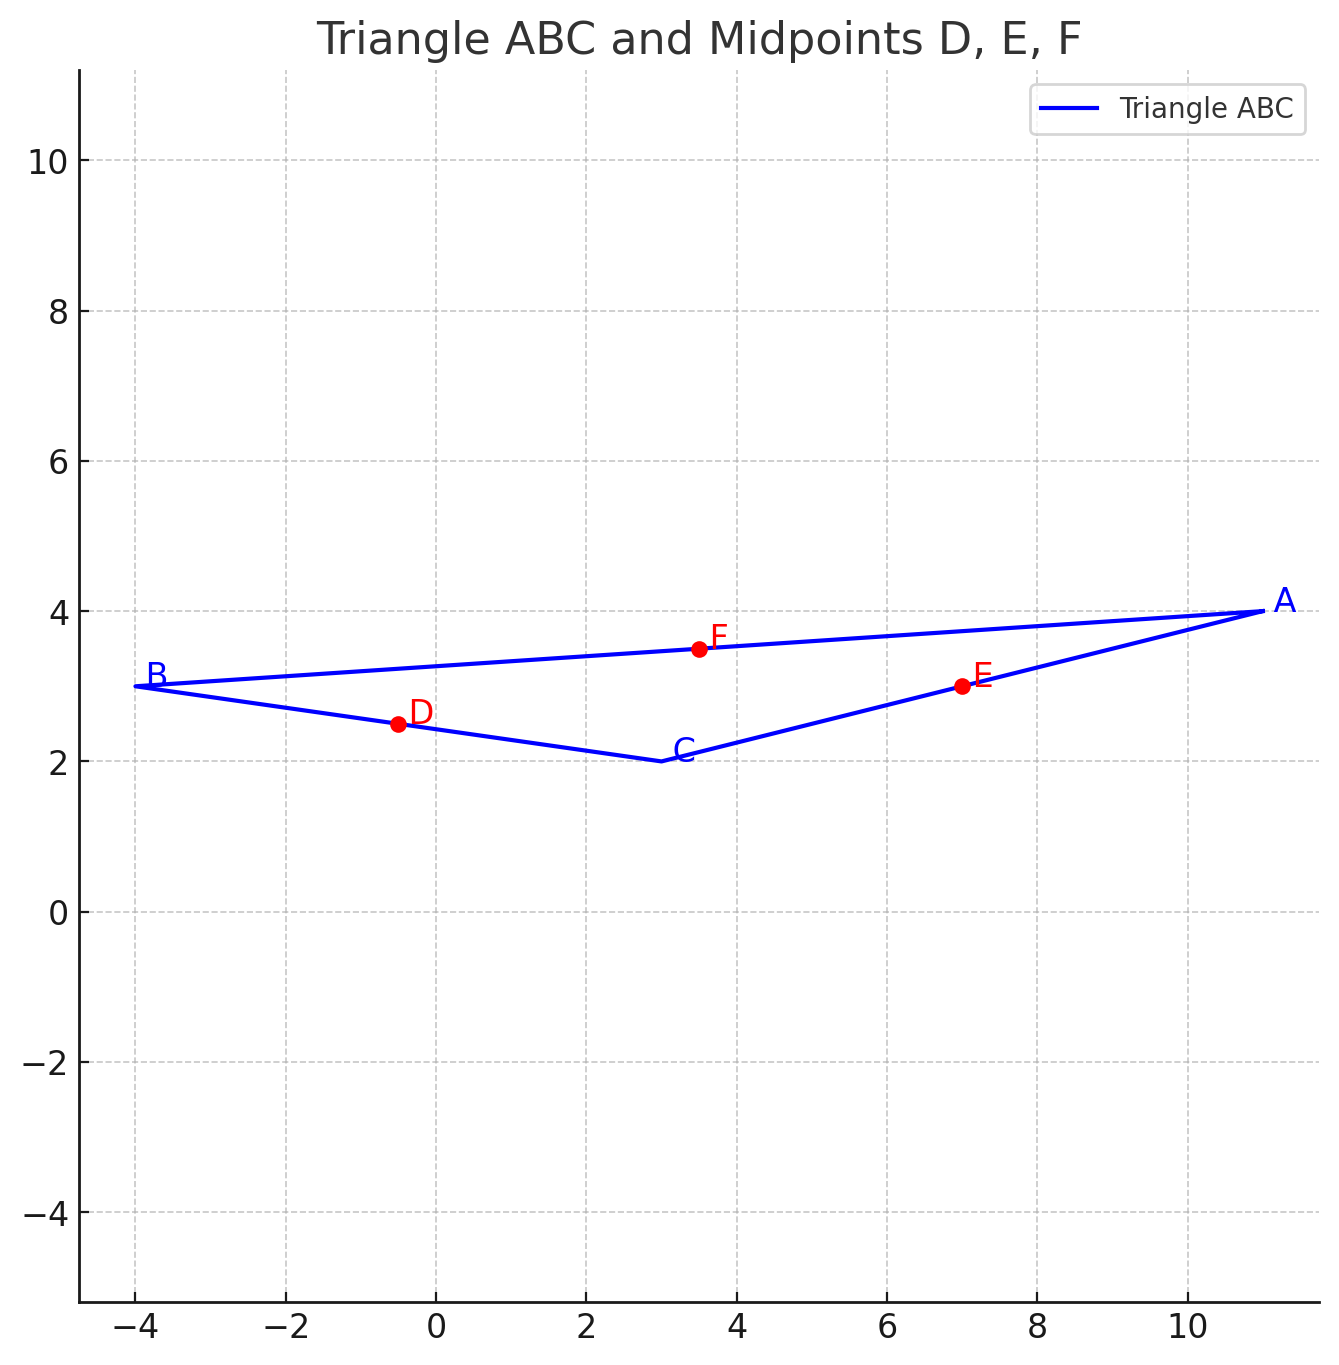
\includegraphics[width=0.7\linewidth]{figs/area.png}
    \caption{Enter Caption}
    \label{fig:placeholder}
\end{figure}
    
\end{frame}
\end{document}